% !TEX TS-program = pdflatex
% !TEX encoding = UTF-8 Unicode

% This is a simple template for a LaTeX document using the "article" class.
% See "book", "report", "letter" for other types of document.

\documentclass[9pt,hyperref]{article} % use larger type; default would be 10pt
\setcounter{secnumdepth}{1}

\usepackage[utf8]{inputenc} % set input encoding (not needed with XeLaTeX)

%\%\% Examples of Article customizations
% These packages are optional, depending whether you want the features they provide.
% See the LaTeX Companion or other references for full information.

%\%\% PAGE DIMENSIONS
\usepackage[margin=1.3in]{geometry} % to change the page dimensions
\geometry{a4paper} % or letterpaper (US) or a5paper or....
% \geometry{margin=2in} \% for example, change the margins to 2 inches all round
% \geometry{landscape} \% set up the page for landscape
%   read geometry.pdf for detailed page layout information

\usepackage{graphicx} % support the \includegraphics command and options

% \usepackage[parfill]{parskip} \% Activate to begin paragraphs with an empty line rather than an indent

%\%\% PACKAGES
\usepackage{hyperref}
\hypersetup{
	colorlinks, linkcolor={red!80!black},
	citecolor={blue}, urlcolor={red!50!black}
}

\usepackage[authoryear]{natbib}
\usepackage{amsmath} % for much better looking tables
\usepackage{xspace}
\usepackage{url}
\usepackage{soul}
\usepackage[table,x11names,dvipsnames]{xcolor}
\usepackage{amssymb} % for much better looking tables
\usepackage{booktabs} % for much better looking tables
\usepackage{array} % for better arrays (eg matrices) in maths
\usepackage{ntheorem} % for better arrays (eg matrices) in maths
\usepackage{paralist} % very flexible & customisable lists (eg. enumerate/itemize, etc.)
\usepackage{verbatim} % adds environment for commenting out blocks of text & for better verbatim
\usepackage{subfig} % make it possible to include more than one captioned figure/table in a single float
\usepackage{mdframed}
\usepackage{relsize}
\usepackage{pgf}
\usepackage{cabin}
\usepackage{enumitem}
\usepackage{tgtermes}
\usepackage{collcell}
\usepackage{adjustbox}% to resize figures

%\usepackage{tgadventor}
% These packages are all incorporated in the memoir class to one degree or another...

%\%\% HEADERS & FOOTERS
\usepackage{fancyhdr} % This should be set AFTER setting up the page geometry
\pagestyle{fancy} % options: empty , plain , fancy
\renewcommand{\headrulewidth}{0pt} % customise the layout...
\lhead{}\chead{}\rhead{}
\lfoot{}\cfoot{\thepage}\rfoot{}

%\%\% SECTION TITLE APPEARANCE
\usepackage{sectsty}
\allsectionsfont{\sffamily\mdseries\upshape} % (See the fntguide.pdf for font help)
% (This matches ConTeXt defaults)

%\%\% ToC (table of contents) APPEARANCE
\usepackage[nottoc,notlof,notlot]{tocbibind} % Put the bibliography in the ToC
\usepackage[titles,subfigure]{tocloft} % Alter the style of the Table of Contents
\renewcommand{\cftsecfont}{\rmfamily\mdseries\upshape}
\renewcommand{\cftsecpagefont}{\rmfamily\mdseries\upshape} % No bold!


\newcommand{\FAnswer}[1]{{\color{black!95}#1}}
\newcommand{\IAnswer}[1]{\FAnswer{\hfill $\to$ #1}}
\newcommand{\PAnswer}[1]{\FAnswer{\\#1}}

\newcommand{\Answer}[1]{\noindent{{{\sffamily Response:} }{\FAnswer{#1}}}}
\newcommand{\Comment}[1]{\item{\color{red!40!black}{{\sffamily Comment:} }{#1}}}
\newcommand{\Quote}[1]{\begin{mdframed}[backgroundcolor=black!2,linecolor=gray!50, linewidth=.6mm]#1\end{mdframed}}

\usepackage[colorinlistoftodos]{todonotes}
\newcommand{\TODO}[2][All]{{\todo[color=blue!10,inline]{\color{black}{TODO (#1)}: #2}}}
\newcommand{\TODOBruno}[2][Bruno]{{\todo[color=red!10,inline]{\color{black}{TODO (#1)}: #2}}}
\newcommand{\TODOAfaf}[2][Afaf]{{\todo[color=Aquamarine3,inline]{\color{black}{TODO (#1)}: #2}}}

%\%\% END Article customizations


%\%\% The "real" document content comes below...


%\%\%\%\%\%\%\%\%\%\%\%\%\%\%\%\%\%\%\%\%\%\%\%\%\%\%\%\%\%\%\%\%\%\%\%\%\%\%\%\%\%\%\%\%\%
%\%                                          \%\%
%\% Enter the authors here                   \%\%
%\%                                          \%\%
%\% Specify information, if available,       \%\%
%\% in the form:                             \%\%
%\%   <key>={<id1>,<id2>}                    \%\%
%\%   <key>=                                 \%\%
%\% Comment or delete the keys which are     \%\%
%\% not used. Repeat \author command as much \%\%
%\% as required.                             \%\%
%\%                                          \%\%
%\%\%\%\%\%\%\%\%\%\%\%\%\%\%\%\%\%\%\%\%\%\%\%\%\%\%\%\%\%\%\%\%\%\%\%\%\%\%\%\%\%\%\%\%\%


%%%%%% TIKZ %%%%%%%%%%%%%%%%%%%%%%%%

\tikzstyle{startend}=[rectangle, rounded corners, minimum width=2cm,  minimum height=1cm, text width =2cm, text centered, draw=none, fill= orange!50, font=\sf]
\tikzstyle{io}=[trapezium, trapezium left angle=70,trapezium right angle= 110,minimum width=3.9cm, minimum height=1cm, text centered, draw=none, fill= blue!30, font=\sf]

\tikzstyle{process}=[rectangle, minimum width=3cm,maximum width=3, minimum height=1cm, text centered, draw=black, fill= orange!30, font=\sffamily]
\tikzstyle{Vprocess}=[rectangle, minimum width=6cm, minimum height=1cm, text centered, font=\sf\bfseries,  fill= gray!80, draw=none, text=white]
\tikzstyle{VSprocess}=[rectangle, minimum width=1cm, minimum height=2cm, text centered, font=\sf\bfseries,  fill= gray!80, draw=none, text=white]
\tikzstyle{squareprocess}=[rectangle, minimum width=2cm, minimum height=7cm, text centered, draw=black, fill= orange!30, font=\sffamily]
\tikzstyle{Bprocess}=[rectangle, minimum width=6cm, minimum height=1cm, text centered,  font=\sf\bfseries,  fill= cyan!60!black, draw=none, text=white]
\tikzstyle{BSprocess}=[rectangle, minimum width=3cm, minimum height=1cm, text centered, draw=black, fill= orange!30, font=\sffamily]
\tikzstyle{decision}=[diamond, minimum width=2.5cm, minimum height=1.5cm, align=center, inner sep=-5pt ,font=\sf\bfseries,  fill= PineGreen!60, draw=none, text=white]
\tikzstyle{IO}=[text=white]

\tikzstyle{arrow}=[line width=1.5pt, ->, >=stealth, gray!80!black]
\tikzstyle{arrowcaption}=[font=\sf\relsize{+1},black]
\tikzstyle{input}=[fill= gray!80!black, inner sep=5pt,rounded corners=5pt]
\tikzstyle{output}=[fill= gray!80!black, inner sep=5pt,rounded corners=5pt]

\pgfkeys{/heat/.is family, /heat,
	Max colour/.initial = Green4,
	Min colour/.initial = Red1,
	max colour/.initial = SpringGreen3,
	mid colour/.initial = white,
	min colour/.initial = Yellow1,
	text colour/.initial = black,
	Min color/.style = {Min colour=#1},% for our friends who can't spell
	Max color/.style = {Max colour=#1},
	min color/.style = {min colour=#1},
	mid color/.style = {mid colour=#1},
	max color/.style = {max colour=#1},
	text color/.style = {text colour=#1},
	min/.initial = -1,
	mid/.initial = 0,
	max/.initial = 1,
	slider/.code={%
		\tikz{\shade[left color=\HVal{min colour},%
			right color=\HVal{max colour}]%
			(current page.south west) rectangle ++(#1,12pt);
		}%
	}%
}

\newcommand{\tikzcircle}[2][red,fill=red]{\tikz[baseline=-0.5ex]\draw[#1,radius=#2] (0,0) circle ;}%
\newcommand\Heatset[1]{\pgfkeys{/heat, #1}}
\newcommand\HVal[1]{\pgfkeysvalueof{/heat/#1}}

\newcolumntype{H}{>{\collectcell\Heat}r<{\endcollectcell}}
\newcommand\Heat[1]{% \Heat{number in the interval [min, max] }
	\if\relax\detokenize{#1}\relax% empty cell
	\else%
	\pgfmathparse{int(100*(#1-\HVal{min})/(\HVal{max}-\HVal{min}))}% map number to [0,100]
	\ifnum\pgfmathresult>100% too big
	\edef\HeatCell{\noexpand\cellcolor{\HVal{Max colour}}}%
	\else\ifnum\pgfmathresult<0% too small
	\edef\HeatCell{\noexpand\cellcolor{\HVal{Min colour}}}%
	\else\ifnum\pgfmathresult<50% between min and mid
	\pgfmathparse{int(2*\pgfmathresult)}% map number to [0,100]
	\edef\HeatCell{\noexpand\cellcolor{\HVal{mid colour}!\pgfmathresult!\HVal{min colour}}}%
	\else% between min and max
	\pgfmathparse{int(2*(\pgfmathresult-50))}% map number to [0,100]
	\edef\HeatCell{\noexpand\cellcolor{\HVal{max colour}!\pgfmathresult!\HVal{mid colour}}}%
	\fi%
	\fi%
	\fi%
	\HeatCell\textcolor{\HVal{text colour}}{$#1$}%
	\fi%
}

\pgfkeys{/heatsec/.is family, /heatsec,
	Max colour/.initial = Green4,
	Min colour/.initial = Red1,
	max colour/.initial = SpringGreen3,
	mid colour/.initial = white,
	min colour/.initial = Yellow1,
	text colour/.initial = black,
	Min color/.style = {Min colour=#1},% for our friends who can't spell
	Max color/.style = {Max colour=#1},
	min color/.style = {min colour=#1},
	mid color/.style = {mid colour=#1},
	max color/.style = {max colour=#1},
	text color/.style = {text colour=#1},
	min/.initial = -1,
	mid/.initial = 0,
	max/.initial = 1,
	slider/.code={%
		\tikz{\shade[left color=\HVal{min colour},%
			right color=\HVal{max colour}]%
			(current page.south west) rectangle ++(#1,12pt);
		}%
	}%
}
\newcommand\HeatSecset[1]{\pgfkeys{/heatsec, #1}}
\newcommand\HSVal[1]{\pgfkeysvalueof{/heatsec/#1}}

\colorlet{BadCol}{Burlywood1!70!red}


\newcolumntype{S}{>{\collectcell\HeatSec}r<{\endcollectcell}}
\newcommand\HeatSec[1]{% \Heat{number in the interval [min, max] }
	\if\relax\detokenize{#1}\relax% empty cell
	\else%
	\pgfmathparse{int(100*(#1-\HSVal{min})/(\HSVal{max}-\HSVal{min}))}% map number to [0,100]
	\ifnum\pgfmathresult>100% too big
	\edef\HeatCell{\noexpand\cellcolor{\HSVal{Max colour}}}%
	\else\ifnum\pgfmathresult<0% too small
	\edef\HeatCell{\noexpand\cellcolor{\HSVal{Min colour}}}%
	\else\ifnum\pgfmathresult<50% between min and mid
	\pgfmathparse{int(2*\pgfmathresult)}% map number to [0,100]
	\edef\HeatCell{\noexpand\cellcolor{\HSVal{mid colour}!\pgfmathresult!\HSVal{min colour}}}%
	\else% between min and max
	\pgfmathparse{int(2*(\pgfmathresult-50))}% map number to [0,100]
	\edef\HeatCell{\noexpand\cellcolor{\HSVal{max colour}!\pgfmathresult!\HSVal{mid colour}}}%
	\fi%
	\fi%
	\fi%
	\HeatCell\textcolor{\HSVal{text colour}}{$#1$}%
	\fi%
}

%%%%%% MACROS %%%%%%%%%%%%%%%%%%%%%%%%

\definecolor{lightsalmon}{rgb}{1.0, 0.63, 0.48}
\definecolor{lightseagreen}{rgb}{0.13, 0.7, 0.67}
\definecolor{americanrose}{rgb}{1.0, 0.01, 0.24}
\DeclareMathOperator*{\argmin}{\arg\!\min}
\DeclareMathOperator*{\argmax}{\arg\!\max}
\newcommand{\multicoomment}[1]{}
\newcommand{\Software}[1]{\text{\ttfamily\bfseries #1}}
\newcommand{\OurTool}{\Software{IPANEMAP}\xspace}
\newcommand{\SM }{{\tt SHAPEMap}\xspace}
\newcommand{\SH }{{\tt SHAPE}\xspace}
\newcommand{\VP }{{\tt Vienna package}\xspace}
\newcommand{\OurRna}{\Software{Did}\xspace}
\newcommand{\mm }{{\tt$M\&M$}\xspace}
\newcommand{\DP }{{\tt DP}\xspace}
\newcommand{\didy }{{\sf GIR1 Lariat-capping ribozyme}\xspace}

\newcommand{\CE }{{\tt capillary electrophoresis}\xspace}
%MPCRnas MultiProbing Conformers}}
% Macros for # variables
\newcommand{\BP }{{\mathcal{ BP}}}
\newcommand{\Ensemble }{{\mathcal{ S}}}
\newcommand{\Sample }{{\mathcal{ S_D}}}
\newcommand{\PData }[1]{{\mathcal{ D}_{#1}}}
\newcommand{\Bzcond}[1]{ \mathbb{P}(s\mid #1)}
\newcommand{\CBP}[1]{ \mathbb{CP}_#1}
\newcommand{\BF}{ \mathbb{BF}}
\newcommand{\Zed}{\mathbb{Z}}
\newcommand{\Edist }{{ \text{Dist}}}
\newcommand{\RL }{{n}}
\newcommand{\CL}{MBkM\xspace}
\newcommand{\Clusters}{\mathcal{C}}
\newcommand{\Centroids}{\mathcal{C_O}}
\newcommand{\GMean}{\text{GM}}
\newcommand{\Ref}{R}
%\newcommand{\OurRna}{\Software{Did}}
%MPCRnas MultiProbing Conformers}}
\newcommand{\NumClust}{k}
\newcommand{\etal}{~\emph{et al} }
\newcommand{\Def}[1]{{\em #1}}

%%% Conditions
\newcommand{\Cond}[5]{\textsc{#1-#3$^{\text{#2}}_{\text{#4}}$#5}}

\newcommand{\OneMSevILUMg}{\Cond{1M7}{mg}{MaP}{il}{}\xspace}
\newcommand{\OneMSevILU}{\Cond{1M7}{}{MaP}{il}{}\xspace}

\newcommand{\OneMSevILUThreeMg}{\Cond{1M7}{mg}{MaP}{il}{-3d}\xspace}
\newcommand{\OneMSevILUThree}{\Cond{1M7}{}{MaP}{il}{-3d}\xspace}

\newcommand{\OneMSevMgCE}{\Cond{1M7}{mg}{CE}{}{}\xspace}
\newcommand{\OneMSevCE}{\Cond{1M7}{}{CE}{}{}\xspace}

\newcommand{\CMCTMg}{\Cond{CMCT}{mg}{CE}{}{}\xspace}

\newcommand{\NMIA}{\Cond{NMIA}{}{MaP}{it}{}\xspace}
\newcommand{\NMIAMg}{\Cond{NMIA}{mg}{MaP}{it}{}\xspace}

\newcommand{\NMIACE}{\Cond{NMIA}{}{CE}{}{}\xspace}
\newcommand{\NMIAMgCE}{\Cond{NMIA}{mg}{CE}{}{}\xspace}

\newcommand{\NAIMg}{\Cond{NAI}{mg}{CE}{}{}\xspace}
\newcommand{\NAICE}{\Cond{NAI}{}{CE}{}{}\xspace}

\newcommand{\BzCN}{\Cond{BzCN}{}{CE}{}{}\xspace}
\newcommand{\BzCNMg}{\Cond{BzCN}{mg}{CE}{}{}\xspace}

\newcommand{\DMSMg}{\Cond{DMS}{mg}{CE}{}{}\xspace}

\newcommand{\BZCNCE}{\Cond{BzCN}{}{CE}{}{}\xspace}


\newcommand{\Draft}[1]{{#1}}
\newcommand{\bs}[1]{\Draft{\todo[color=red!30]{\sf Bruno: #1}}}
\newcommand{\bsi}[1]{\Draft{\todo[color=red!30,inline]{\sf Bruno: #1}}}
\newcommand{\as}[1]{\Draft{\todo[color=green!70!black]{\sf Afaf: #1}}}
\newcommand{\yp}[1]{\Draft{\todo[color=blue!30]{\sf Yann: #1}}}
\newcommand{\ypi}[1]{\Draft{\todo[color=blue!30,inline]{\sf Yann: #1}}}

%\renewcommand{\bsi}[1]{}
%\renewcommand{\ypi}[1]{}

\newcommand{\ipanemapurl}{https://github.com/afafbioinfo/IPANEMAP}

\newcommand{\Bull}[1]{{\sffamily #1}~\raisebox{1pt}{\tikzcircle[black, fill=cluster#1]{3pt}}}

\newcommand{\BullLab}[1]{Cluster \Bull{#1}}

\colorlet{clusterA}{SeaGreen}
\colorlet{clusterB}{Yellow}
\colorlet{clusterC}{gray}
\definecolor{clusterD}{HTML}{AFAFE9}
\colorlet{clusterE}{OliveGreen}
\colorlet{clusterF}{blue!90!black}
\colorlet{clusterG}{Orange}
\colorlet{clusterH}{SeaGreen!40}


\title{Response to second round of reviews\\[.3em]\OurTool{}:  Integrative Probing Analysis of Nucleic Acids Empowered by Multiple Accessibility Profiles}
\author{
Afaf Saaidi \and
Delphine Allouche \and
Mireille Regnier \and
Bruno Sargueil \and
Yann Ponty}

\date{} % Activate to display a given date or no date (if empty),
         % otherwise the current date is printed 

\begin{document}
\maketitle

%\tableofcontents

%\section{Specific responses}

	\subsection{Reviewer \#4}
	\begin{enumerate}[resume]
\Comment{The revised manuscript is much clearer now. However, I am still puzzled over the performance comparison between IPANEMAP and Rsample over Hajdin et al.’s data. The Hajdin dataset consists of 24 RNAs, but only 16 of them were considered in the Rsample paper (per its supplementary information). As I previously commented, IPANEMAP’s performance gains are really dramatic for the few sequences that were not considered by Spasic et al. For example, 5SrEcoli, signal recognition particle, and E. coli tRNA(phe). 

Nevertheless, I also looked at a few of the sequences considered by both Spasic et al. and the authors. Below are a few examples of inconsistencies between these two benchmarks:

[..]


Can the authors reconcile these discrepancies, or alternatively, am I missing something in the way this benchmark was set up? }

    \Answer{We had indeed spotted these discrepancies, which we had initially attributed to code differences between the versions of \Software{RSample} used in the initial benchmark, and the one currently available online. 
    
	Following this reviewer's remark, we have corresponded with the authors of \Software{RSample}, and discovered the origin of the discrepancy. Namely, we had made the erroneous assumption that the format used to specify reactivities in \Software{RSample} was similar to the one used in the \Software{Vienna} package. Instead, the reactivity file format used in \Software{RSample} requires three columns per position, and we discovered that \Software{RSample} silently fails if a poorly-formatted file is provided. In this case, it \Def{reverts to a reactivity-free prediction} (essentially, an MEA prediction). It follows that the results reported for \Software{RSample} in the initial versions of the manuscript were those of a purely thermodynamic prediction, and did not reflect \Software{RSample}'s  performances when informed by reactivity data.
	
	When informed by suitably-formatted reactivities files, \Software{RSample} now predicts structures having accuracy that are much closer to those reported in \citet{Spasic2017}. \OurTool still appears to outperform \Software{RSample} slightly, reporting more accurate structures than its competitor for roughly two thirds of the tested RNAs. However, its average improvement in term of Geometric Mean is only of around 1.5\% over the \citet{Hajdin2013} dataset, an improvement that is no longer significant according to a two-tailed T-test with paired data. Upon, multiple executions of \Software{RSample}, we have witnessed minor variations, but always a slightly inferior (yet insignificant) average GM that the one of \OurTool.
	
	We have replaced the erroneous content in our revised version, including the above Figure, and have toned down the relevant subsection to reflect our new assessment. Similarly, we have removed from the conclusion our discussion on the possible origins of the discrepancy in performances.
	
	We are greatly indebted to this reviewer for following through on this point, allowing us to fix our initial (involuntary) misrepresentation of the predictive capacities of \Software{RSample}.
	
	\begin{figure}[t]
		
	{\centering 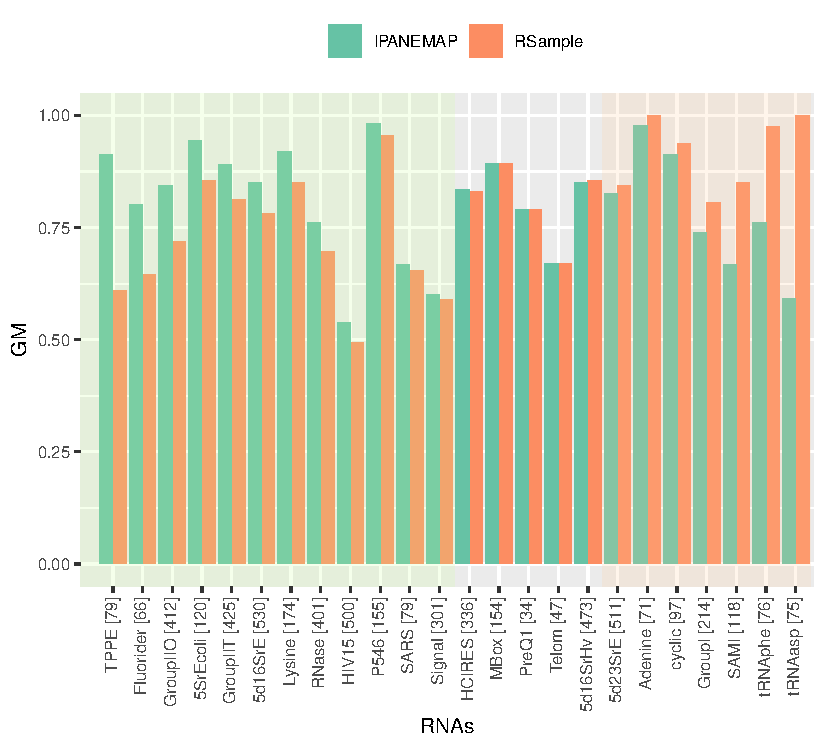
\includegraphics[width=.8\textwidth]{graphs/RsampleVsIPANEMAP/Accuracy.pdf}\\}

	\caption{Updated figure presenting the geometric means of structures predicted by \OurTool (green) and \Software{RSample} (orange -- corrected).}
	\end{figure}}

	\Comment{Additionally, referring to the authors comment on page 24: “we object to such an adversarial view of this particular analysis (and, more generally, our work)…”  I would like to clarify I had no such intention. My critique aimed at strengthening or solidifying the reported results. I am sorry the authors interpreted my requests for better controls and comparisons as a negative opinion of their work.}

	\Answer{In addition to erring in our comparison against \Software{RSample}, we also expressed ourselves poorly in this instance. It is, of course, entirely legitimate to request more tests and benchmarks and, possibly (but not ideally) to express a negative opinion of our work (peer-review is a pillar of the academic world). We merely wished to express disagreement with what we interpreted as a request to demonstrate domination over \Software{RSample}. Our resistance was essentially inspired by the almost anecdotal nature of the performances of \OurTool{} in the single probing setting, here presented as a sanity check rather than a central point of our study.}
	\end{enumerate}


	\subsection{Reviewer \#3}

		\begin{enumerate}[resume]
	\Comment{On page 4, in “Cordero dataset”, the text states that the reactivity is set to 0 for nucleotide identities that are unreactive to a specific probing agent.  But 0 is a reactivity that receives a negative pseudoenergy free change, encouraging base pairing.  It would be much better to give a 0 pseudo free energy change.  Is it possible the manuscript should really state a 0 free energy change?  If not, the authors should add some text to justify this choice.}
	
    \Answer{Indeed, we set the pseudo-energy to 0 (and not the reactivity, as erroneously stated in the manuscript). This is now corrected in the revised manuscript.}
	
	\Comment{On page 4, the text states “a standard denaturation protocol”, but I think the manuscript should state “a standard annealing protocol”.  It looks like the intent was to anneal the structure to find its equilibrium structure at 37 degrees C, not to leave the structure denatured.}    
    
    \Answer{Indeed, our denomination was arguably lacking in precision. While the term "annealing" would be entirely acceptable, we prefer to use "denaturation/renaturation protocol", as it currently represents the standard nomenclature.}
    
	\Comment{On page 5, in statistical significance, “usual significance threshold” should really state the “usual type I error rate”.  Alpha is the probability of falsely rejecting the null hypothesis (type I error).  “Threshold” doesn’t convey this meaning.  }
    
    \Answer{We thank the reviewer for suggesting this more precise formulation, which we adopted in this revision.}
    
	\Comment{On page 8, “barely significant” should just be changed to “but significant”. The improvements may be modest, but they are significant.  I don’t agree that something can be “barely” significant.}
    
    \Answer{We respectfully disagree with this statement: an observation that would be deemed significant for $\alpha=5\%$, but not $\alpha=1\%$ should arguably be described as more weakly supported, on a statistical level, than an observation supported for both type I error rates. This is reflected by the qualifier "barely" in this context.}
    
	\Comment{On page 10, “Considering three conditions yields improvement over the average performance of the triplet” confuses me.  I think what was intended is “Considering three conditions yields improvement over the average performance of the doublet [/pair]” }
	
    \Answer{The main result of this section is that, when considering a triplet of conditions, the average performance of prediction informed by individual conditions, is lower than that of predictions simultaneously informed by the three conditions. We modified the title of this subsection to "Considering three conditions yields improvement over the average of single conditions in the same triplet", hoping this will be more explicit to the reader.}
	\end{enumerate}

	\subsubsection{Typos:}
	
	\begin{enumerate}[resume]
	\Comment{On page 1, “different dynamics, that can help” should be “different dynamics that can help”.}
	
	\Answer{Fixed}
	\Comment{On page 3, “using an iterative heuristics” should be “using an iterative heuristic”.  Also, “we elect the most promising cluster” should be “we select the most promising cluster”.}
	
	\Answer{Fixed}
	\Comment{On page 6, “Spacic” should be “Spasic”.}
	
	\Answer{Fixed}
	\end{enumerate}

\subsubsection{Suggestions:}

\begin{enumerate}[resume]
	\Comment{On page 1, there is a new phrase about probes “some of which are usable in vivo”.  My recollections is that Zaug and Cech were the first to demonstrate in vivo probing of RNA structure, and it is probably worth citing the paper [RNA. 1995 1:363.].}

	\Answer{We added a reference to this work, and to a posterior effort more similar to our context of analysis.}
	\Comment{Page 1 claims that using multiple data sources has never been fully automated.  I agree that it has never been automated when using quantitative data and soft constraints.  On the other hand, the deprecated hard constraint method (reference 2) was fully automated and used multiple probing methods.  The phrase should be made more specific.}
	
	\Answer{We qualified this statement by mentioning explicitly, and adding a reference to the soft constraint framework. 
		
		However, we feel the statement holds more generally as far as the automation is concerned, since the hard constraint framework makes it virtually impossible to integrate multiple type of probing data in an automated way. Indeed, hard constraints are obtained from reactivities based on cutoffs, whose values are somewhat arbitrary. Overly liberal cutoffs will often induce contradictory constraints (i.e. no compatible structure) across experiments, while conservative cutoffs will lead to sparse constraints, leading to a waste of most of the probing-derived information. 
		
		In fact the tediousness, and suboptimality, of manually selecting those cutoffs while modeling HIV-1 structural elements~\citep{Deforges2017}, was one of the main motivation for this work.}

	\end{enumerate}


\bibliographystyle{abbrvnat}
\bibliography{biblio}
\end{document}
